\documentclass[a4paper,twoside]{article}

\usepackage{epsfig}
\usepackage{graphicx}
\usepackage{subcaption}
\usepackage{calc}
\usepackage{amssymb}
\usepackage{amstext}
\usepackage{amsmath}
\usepackage{amsthm}
\usepackage{multicol}
\usepackage{pslatex}
\usepackage{natbib}
\usepackage{algorithm2e}
\usepackage[bottom]{footmisc}
\usepackage{SCITEPRESS}
\usepackage[hidelinks]{hyperref}

\begin{document}

\title{Dataset, Methodology, and Results: A Bilingual Hybrid-Retrieval Academic Advising System}

\author{\authorname{Anonymous Author(s)}
\affiliation{Anonymous Institute}
\email{anonymous@anonymous.edu}
}

\keywords{Retrieval-Augmented Generation, Hybrid Retrieval, Dataset Construction, Academic Advising, Code-Mixed NLP, Evaluation Methodology.}

\abstract{This report documents, in one place, the dataset, the research process, and the full results behind a bilingual (English/Banglish) hybrid-retrieval academic-advising system. The corpus comprises 7{,}138 indexed chunks drawn from 5{,}429 curated question-answer pairs (2{,}385 English, 3{,}044 Banglish, including a naturally-occurring 190-row Out-of-Scope/Unanswerable category used as a real should-abstain label set) and 1{,}709 structured institutional records across five administrative tables. We describe the dataset's provenance and construction, the verified chronological arc of methodology decisions that shaped the deployed system, and every result obtained -- headline novelty findings, retrieval quality, generation faithfulness, an abstention-gate accuracy progression from 0.612 to 0.737, a five-configuration reranker ablation, a four-model independent faithfulness cross-check, and efficiency/robustness measurements -- with paired statistical significance testing applied throughout and every reported number traceable to a script that produced it.}

\onecolumn \maketitle \normalsize \setcounter{footnote}{0} \vfill

\section{\uppercase{Introduction}}
\label{sec:introduction}

Academic advising at open-credit institutions places substantial demands on students to independently interpret policy, plan course sequences, and resolve entity-specific questions (course codes, prerequisite chains, faculty records) -- demands compounded when a meaningful share of student questions arrive not in formal English but in Banglish, Bengali-English code-mixed text typed in Latin script. This report is a focused companion to the full system paper, organized around three questions rather than the system's novelty claims: what data was this system built and evaluated on, what process produced its current configuration, and what did every evaluation actually measure. We treat these as reporting obligations independent of any single headline result -- a dataset section a reviewer can audit, a methodology section that shows real dead ends alongside real fixes, and a results section that omits nothing that was actually measured, including the results that did not work out.

Three standing conventions govern everything reported below. First, every number traces to a script that was actually executed and an output file it produced -- nothing here is an estimate. Second, every statistical claim of significance requires agreement between two different paired tests (a parametric paired $t$-test and a non-parametric Wilcoxon signed-rank test); when they disagree, the result is reported as inconclusive, never rounded up to a confirmed finding. Third, negative and null results are retained and reported with the same care as positive ones -- five reranker configurations and three of four faithfulness cross-check models did not improve on what came before them, and all are documented here rather than quietly omitted.

\section{\uppercase{Dataset}}
\label{sec:dataset}

\subsection{Overview and Scale}
\label{subsec:dataset-overview}

The corpus totals \textbf{7{,}138} indexed chunks, built from two kinds of source material: curated bilingual question-answer pairs (5{,}429 rows) and structured institutional administrative records (1{,}709 rows) across five tables. Table~\ref{tab:dataset-overview} summarizes the composition; every count below was queried directly from the deployed SQLite knowledge base and the corpus's own chunked JSONL file, not estimated.

\begin{table}[h]
\caption{Corpus composition by source table.}\label{tab:dataset-overview}\centering
\begin{tabular}{|l|c|c|}
\hline
Source & Rows & Chunk share \\
\hline
BanglishQA & 3{,}044 & 42.7\% \\
EnglishQA & 2{,}385 & 33.4\% \\
FacultyAvailability & 814 & 11.4\% \\
CourseDetails & 586 & 8.2\% \\
FacultyList & 223 & 3.1\% \\
Coordinator & 52 & 0.7\% \\
Prerequisites & 34 & 0.5\% \\
\hline
\textbf{Total} & \textbf{7{,}138} & \textbf{100\%} \\
\hline
\end{tabular}
\end{table}

\subsection{EnglishQA}
\label{subsec:englishqa}

EnglishQA contains 2{,}385 rows across 16 topic categories, each tagged with a \texttt{Category}, a \texttt{Type} (Original / Paraphrase / Multi-Hop-Reasoning), a \texttt{Register} describing provenance, and a \texttt{Split} (train/validation/test). Category sizes are near-uniform (129--156 rows) with two structural exceptions: Transportation and Bus Services (129, a genuinely smaller real-world topic) and, by design, Out of Scope / Unanswerable (127).

\textbf{Type breakdown.} 1{,}295 rows are paraphrases of an underlying fact (used for paraphrase-robustness testing), 1{,}071 are original fact statements, and 19 are multi-hop reasoning questions requiring a chain across records (used to evaluate prerequisite-graph traversal).

\textbf{Register (provenance) breakdown.} 1{,}182 rows are student-submitted questions from the original dataset; 969 are synthesized directly from official or secondary university sources; 127 are synthetic negative examples (deliberately unanswerable, paired with the Out-of-Scope category); 88 are LLM-generated, diversity-filtered paraphrases of synthesized facts; and 19 are synthesized multi-hop questions. This provenance labeling means every row's origin is known and auditable, not a black-box scrape.

\textbf{Split.} 1{,}872 train / 235 validation / 278 test, enforced strictly for embedding fine-tuning (Section~\ref{subsec:process-arc}): validation and test rows are never used in training.

Table~\ref{tab:englishqa-categories} gives the full category breakdown.

\begin{table}[h]
\caption{EnglishQA by category ($n=2{,}385$).}\label{tab:englishqa-categories}\centering
\begin{tabular}{|l|c|}
\hline
Category & Rows \\
\hline
Exams and Grading & 156 \\
University Facts \& Governance & 154 \\
Policies and Procedures & 154 \\
Campus & 154 \\
Thesis and Internship & 153 \\
Payment, Financial Aid and Scholarship & 153 \\
Technical Support & 152 \\
Admission & 152 \\
TARC/RS (Residential Semester) & 151 \\
International Student & 151 \\
Programs \& Departments & 150 \\
Library & 150 \\
Extracurricular Activities & 150 \\
Advising & 149 \\
Transportation and Bus Services & 129 \\
Out of Scope / Unanswerable & 127 \\
\hline
\end{tabular}
\end{table}

\subsection{BanglishQA}
\label{subsec:banglishqa}

BanglishQA contains 3{,}044 rows across 17 categories, with a substantially different distribution from EnglishQA: General/Web FAQ dominates at 832 rows, reflecting genuine Banglish usage patterns skewing toward informal, general queries rather than English's more even topical spread. Split: 2{,}414 train / 323 validation / 307 test. Table~\ref{tab:banglishqa-categories} gives the full breakdown.

\begin{table}[h]
\caption{BanglishQA by category ($n=3{,}044$).}\label{tab:banglishqa-categories}\centering
\begin{tabular}{|l|c|}
\hline
Category & Rows \\
\hline
General / Web FAQ & 832 \\
Advising & 273 \\
Policies and Procedures & 264 \\
Programs \& Departments & 261 \\
Admission & 227 \\
Campus & 183 \\
Library & 155 \\
Transportation and Bus Services & 154 \\
TARC/RS (Residential Semester) & 151 \\
Extracurricular Activities & 116 \\
Exams and Grading & 87 \\
Technical Support & 80 \\
Payment, Financial Aid and Scholarship & 76 \\
Out of Scope / Unanswerable & 63 \\
Thesis and Internship & 62 \\
International Student & 38 \\
University Facts \& Governance & 22 \\
\hline
\end{tabular}
\end{table}

The two languages' category distributions differ structurally, not just in scale: EnglishQA is deliberately near-uniform across topics (a curated design choice), while BanglishQA's heavy skew toward General/Web FAQ (27\% of all Banglish rows) reflects how Banglish questions actually arrive in practice -- informal, general-purpose queries rather than the more evenly-distributed formal topic coverage of the English set. This is disclosed as a genuine corpus-design asymmetry, not normalized away.

\subsection{Structured Administrative Tables}
\label{subsec:structured-tables}

Five tables hold the institution's own administrative records -- not scraped or synthesized -- providing exact-match ground truth for entity-heavy queries (course codes, faculty emails, office rooms, prerequisite chains). Table~\ref{tab:structured-schemas} lists each with its row count and schema.

\begin{table}[h]
\caption{Structured table schemas.}\label{tab:structured-schemas}\centering
\begin{tabular}{|l|c|p{4.2cm}|}
\hline
Table & Rows & Key fields \\
\hline
FacultyAvailability & 814 & Initial, Name, Programme, Email, Semester, Room, Day, ScheduleText \\
CourseDetails & 586 & Course, Theory/Lab Equivalent, Theory/Lab Initial/Day/Time/Room, ContactEmail \\
FacultyList & 223 & Initial, Name, Designation, Status, Room, Email \\
Coordinator & 52 & Course, First/Second/Third Theory/Lab Coordinator, Theory/Lab Email \\
Prerequisites & 34 & Course, PreRequisite, FullChainPreRequisite \\
\hline
\end{tabular}
\end{table}

The \texttt{Prerequisites} table's \texttt{FullChainPreRequisite} field is the direct source for the prerequisite-graph traversal mechanism: a directed graph is built from this table's own edge data, not inferred, so multi-hop questions ("what do I need before X's prerequisite") are answered by graph traversal rather than hoping a single retrieved chunk states the full chain.

\subsection{Corpus Construction and Chunking}
\label{subsec:corpus-construction}

Each source table is ingested independently into a relational SQLite store (for structured access and auditability) and separately chunked and embedded into ChromaDB (for semantic search). Chunk size is 2{,}000 characters with 50-character overlap, chosen to comfortably cover this corpus's own measured row-length distribution (p99 $\approx$ 1{,}350 characters) so that multi-chunk splitting within a single row is rare, not the norm. Chunking is performed independently per source table -- rows from different tables are never concatenated together before chunking. Each chunk carries metadata (source table, course code, section, and source question text where applicable), which is what enables exact-match lookup and a question-field-aware similarity boost at retrieval time. A SHA-256 content hash is compared against already-indexed records on every ingestion run, so unchanged content is skipped rather than re-embedded, keeping routine updates fast.

\subsection{Test Set Construction}
\label{subsec:testset-construction}

The main evaluation set is 200 English and 100 Banglish queries with reference answers, drawn from the held-out test splits described above -- never seen during embedding fine-tuning. Reference-answer verification differs by query type: entity-heavy reference answers are composed directly from structured fields (a course code, an email address, a coordinator name) and verified by field-level matching against retrieved candidates, not substring search; open-ended reference answers are the corpus's own verbatim EnglishQA/BanglishQA answer text, verified by substring containment in the candidate chunk. Two smaller, purpose-built subsets support specific ablations rather than constituting independent data collections: a 13-fact cross-lingual stress test (Banglish queries about content that exists only in EnglishQA) and a 60-example entity-heavy abstention calibration set (18 naturally-occurring examples augmented with database-verified synthetic course-code/faculty-initial examples). Both were verified this project as genuine hard data ceilings -- no further naturally-occurring examples exist to add -- rather than left unexamined.

\section{\uppercase{Methodology and Process}}
\label{sec:methodology}

\subsection{System Architecture, Briefly}
\label{subsec:architecture-brief}

The deployed pipeline routes every query as entity-heavy or open-ended before retrieval, then fuses a BM25 stream (\texttt{rank\_bm25}, retuned $k_1=1.5$, $b=0.4$) and a dense stream (a domain-fine-tuned sentence-transformer, base architecture \texttt{all-MiniLM-L6-v2}, 384-dim, contrastively trained via \texttt{MultipleNegativesRankingLoss} on this corpus's own hard negatives) via linear combination, $\mathrm{Score} = \lambda \cdot S_{\mathrm{bm25}} + (1-\lambda) \cdot S_{\mathrm{vec}}$, with adaptive per-route weighting ($\lambda_{\mathrm{entity}}=0.9$, $\lambda_{\mathrm{open}}=0.5$). An optional cross-encoder reranking stage is disabled by default (Section~\ref{subsec:results-reranker}).

\begin{figure}[h]
\centering
{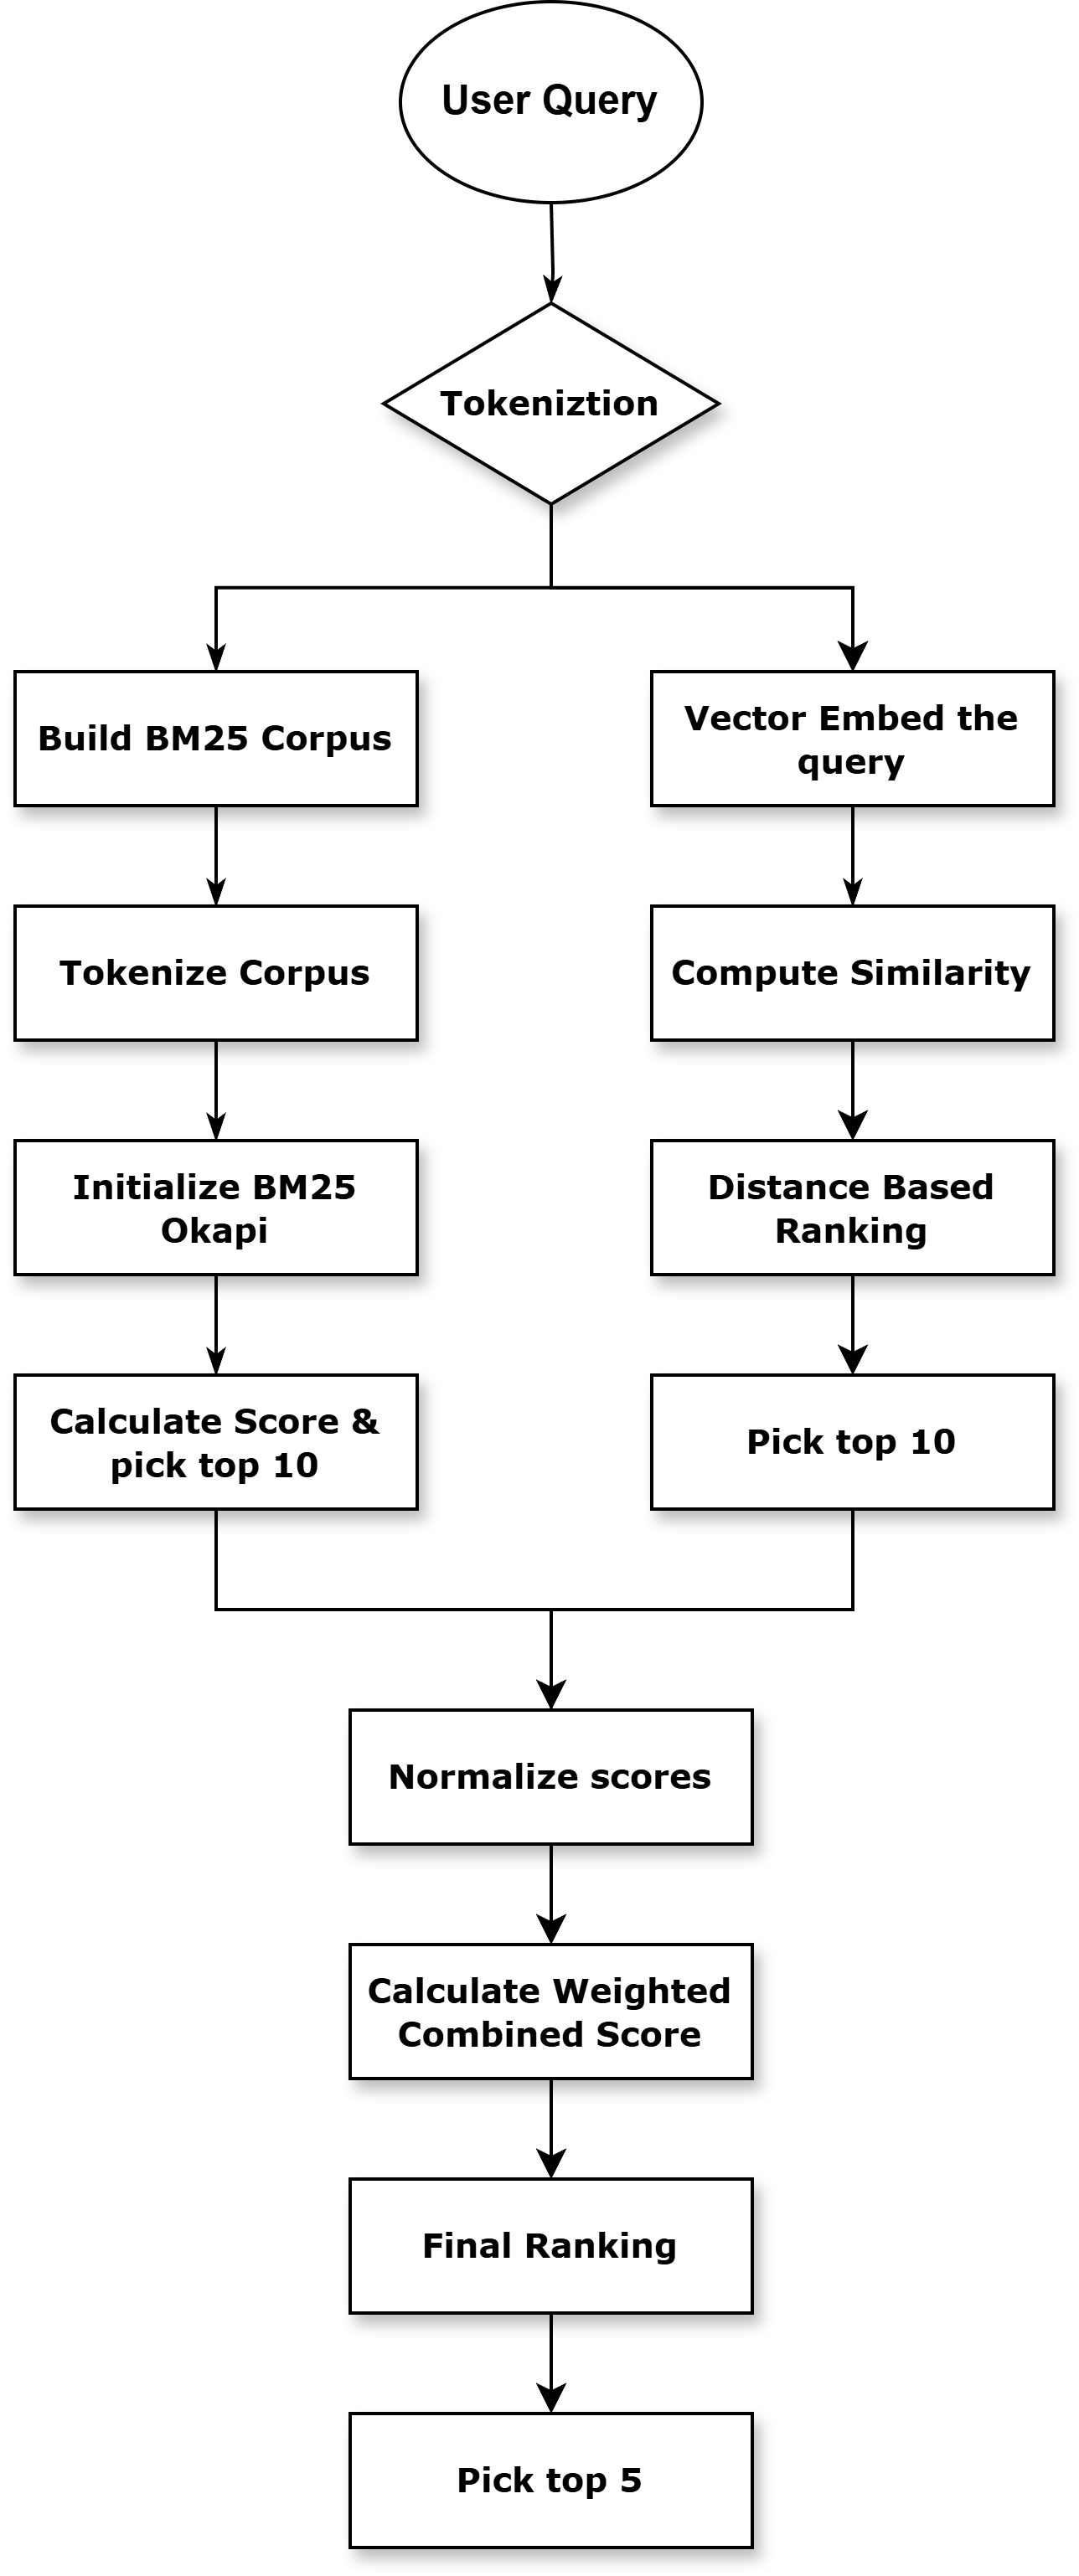
\includegraphics[width=8cm]{fig_hybrid_retriever.png}}
\caption{Base retriever workflow: parallel BM25 and vector retrieval streams merged by weighted score fusion; adaptive routing selects between two fusion configurations of this same mechanism per query type.}
\label{fig:retriever-report}
\end{figure} Context is assembled in confidence-ordered ``zig-zag'' fashion before generation by a locally-served Llama-3.1-8B model (temperature $0.0$, fixed seed $42$). A confidence-gated abstention mechanism, calibrated separately per route, can decline to answer when retrieval confidence is low, subject to a one-directional sufficient-context override that can only ever reduce abstention when direct structural evidence (an exact match, a graph traversal result) is already available.

\subsection{Evaluation Methodology and Statistical Discipline}
\label{subsec:eval-methodology}

Four statistical testing conventions apply throughout every result in Section~\ref{sec:results}, chosen for the specific structure of each measurement type rather than applied uniformly by default:

\begin{itemize}
  \item \textbf{Binary IR metrics} (Recall@$k$, in McNemar-style discordant-pair comparisons): McNemar's exact test on discordant query pairs, cross-checked against a paired bootstrap (2{,}000 resamples).
  \item \textbf{Generation-quality/faithfulness metrics} (BLEU, ROUGE-L, BERTScore, METEOR, faithfulness scores): a paired $t$-test and a Wilcoxon signed-rank test, following \citet{dror2018hitchhiker}'s guidance that graded, potentially non-normally-distributed measures should not rely on an assumed-normal test alone.
  \item \textbf{Cross-validated classifier accuracy} (the abstention gate): 5-fold cross-validation repeated across 5 independent fold-assignment seeds (25 total train/test folds), with the classifier's own random-state stability checked separately from the fold-assignment robustness check.
  \item \textbf{The standing rule}: whenever the two paired tests for a given comparison disagree, the result is reported as inconclusive. This occurs several times in Section~\ref{sec:results} (e.g.\ METEOR vs.\ vector-only retrieval) and is never silently resolved in whichever direction looks more favorable.
\end{itemize}

\subsection{The Verified Fix Arc}
\label{subsec:process-arc}

The deployed system is the result of a chronological sequence of real, individually-tested fixes, not a single design pass. Table~\ref{tab:fix-arc} summarizes the sequence; each row was verified independently before being trusted; several were only found by deliberately testing an assumption rather than accepting an ambiguous result.

\begin{table}[h]
\caption{The verified methodology arc, in order.}\label{tab:fix-arc}\centering
\begin{tabular}{|p{3.1cm}|p{7.6cm}|}
\hline
Step & What was found and done \\
\hline
Exact-match coverage gap & Course-code lookup silently missed an entire table (section-suffixed codes in CourseDetails); fixed by canonicalizing every table under one code format. \\
BM25 retuning & Library defaults ($k_1=1.5$, $b=0.75$) had never been verified against this corpus; retuned to $b=0.4$ after direct testing. \\
Embedding fine-tuning & Off-the-shelf MiniLM adapted via contrastive training on this corpus's own (question, answer) pairs and real retriever-derived hard negatives. \\
Deconfounding diagnostic & Found that adaptive routing's original RRF fusion choice for entity-heavy queries was significantly \emph{worse} (not neutral) once a masking exact-match ranking guarantee was isolated out (Section~\ref{subsec:results-novelty}); replaced with linear fusion, verified no regression. \\
Same-entity ranking bonus & Root-caused a residual nDCG gap to three real faculty members sharing a first name; fixed with a small, safety-verified bonus that can only reorder candidates below an already-guaranteed winner. \\
Cross-process determinism fix & Found while testing an unrelated reranker change: Python's per-process hash randomization made tied candidates non-reproducible across separate runs; fixed with a deterministic secondary sort key, verified via SHA-256 hash matching across 5 runs. \\
Abstention gate, three stages & 0.612 (single threshold) $\to$ 0.644 (4-signal logistic regression) $\to$ 0.737 (gradient-boosted trees) -- each stage cross-validated across 5 independent fold seeds; the final stage additionally checked for overfitting (in-sample vs.\ cross-validated accuracy gap) and classifier-seed stability before deployment. \\
Reranker, five configurations & Generic $\to$ fine-tuned $\to$ pool-restricted $\to$ route-conditional $\to$ route-conditional+pool-restricted. Each a real, separately-tested configuration; all five top out at a tie, never a win. \\
Faithfulness cross-check, four models & MiniLM $\to$ DeBERTa-base $\to$ DeBERTa-large-FEVER (moved to GPU after a 9-hour CPU performance anomaly) $\to$ MiniCheck (blocked by an unresolved dependency/security constraint, not forced through). Root cause of the remaining gap quantified by direct row-level inspection. \\
\hline
\end{tabular}
\end{table}

\subsection{Differentiation from the Closest Related System}
\label{subsec:differentiation}

BanglAssist \citep{kruk2025banglassist}, a Bengali-English code-switching customer-service chatbot, is the closest published system to this project's setting, so novelty cannot be assumed by domain (bilingual, code-switched, retrieval-augmented) alone. Three axes of direct comparison: \textbf{retrieval architecture} -- BanglAssist retrieves with a vector-only index reranked by a generic cross-encoder and translates every query to English before retrieval, whereas this system retrieves with true hybrid BM25+dense fusion directly over Banglish text, a design motivated directly by this project's own ablations showing that a generic reranker and translation-before-retrieval both fail to help on this corpus (Section~\ref{subsec:results-reranker}); \textbf{evaluation rigor} -- BanglAssist evaluates on 20 queries with qualitative scoring and no significance testing, against 300 queries here with paired significance testing throughout; and \textbf{entity disambiguation and calibrated abstention}, the most substantive gap -- BanglAssist's only confidence-adjacent component is a fixed cosine-similarity threshold with no handling for an ambiguous entity reference and no calibrated decline, precisely the gap \texttt{conditioning\_v2} and the confidence-gated abstention gate (Section~\ref{subsec:results-abstention}) are built to close. This is also a domain-shaped gap, not an incidental one: BanglAssist's customer-support setting does not require reasoning over structured, collision-prone entities (course codes, prerequisite chains, faculty records with shared initials) the way academic advising does -- the two facts together, not comparison alone, are why this is treated as a genuine differentiator.

\subsection{Two Fixes Worth Narrating in Full}
\label{subsec:fix-narratives}

Two entries in Table~\ref{tab:fix-arc} illustrate the project's general discipline of testing an assumption directly rather than accepting an ambiguous result, and are worth the additional detail.

\textbf{The cross-process non-determinism bug.} While testing a route-conditional reranker configuration, a control comparison that should have been byte-identical across two separate script invocations instead differed on 49 of 101 entity-heavy queries -- in some cases substantively (e.g.\ one run's retrieved context read ``Day: Tuesday'', the other ``Day: Sunday'', for the identical query and identical candidate documents). The root cause traced to \texttt{hybrid\_retriever.py}'s final ranking step sorting candidates by score alone: when multiple candidates tie exactly (several \texttt{FacultyAvailability} rows for the same person on different days, scoring identically for a query that does not specify a day), Python's stable sort preserves whatever order the candidates happened to arrive in, which traces back to iterating a \texttt{set} of candidate IDs -- and Python randomizes its hash seed for string keys per \emph{process} by default, so two separate invocations of the identical script, on the identical query, corpus, and model, could silently return a different tied candidate first. The fix added a deterministic secondary sort key (candidate \texttt{doc\_id}) to the existing score-based sort; verification used SHA-256 hash matching of the assembled context across five separate process invocations, confirming byte-identical output, and the discrepancy rate on a fresh comparison dropped from 49/101 to 2/101 (the residual two attributable to a much smaller, separately-documented source: floating-point non-determinism in GPU-based generation itself, producing minor paraphrase-level differences in otherwise-correct answers).

\textbf{The abstention gate's third stage, scrutinized harder because it looked too good.} Moving from a 4-signal logistic regression (0.644 cross-validated accuracy) to a gradient-boosted-tree ensemble over the identical four signals produced a jump to 0.737 -- both paired significance tests essentially maximal ($p<0.0001$). A result this clean was treated with more scrutiny, not less, before being deployed: in-sample (full-data) accuracy was checked against the cross-validated figure (0.873 vs.\ 0.737, a normal, moderate gap consistent with genuine generalization rather than the near-100\%/near-chance pattern that would indicate memorization), and the result was re-checked across five different classifier random seeds, independent of the five cross-validation fold-assignment seeds already used to validate it (0.7374--0.7390, effectively identical, ruling out a lucky-seed artifact of the tree algorithm's own internal randomness). Only after both checks passed was the classifier fit on the full calibration set and deployed.

\subsection{Tools and Models}
\label{subsec:tools}

Generation: Llama-3.1-8B served locally via Ollama. Dense retrieval: a contrastively fine-tuned sentence-transformer (base \texttt{all-MiniLM-L6-v2}). Sparse retrieval: \texttt{rank\_bm25}. Reranking (disabled by default): an MS-MARCO-tuned MiniLM cross-encoder ($\sim$33M parameters), also tested after fine-tuning on this corpus's own hard negatives. Faithfulness cross-check: four independent NLI/grounding-verification models (Section~\ref{subsec:results-faithfulness}). Classifiers: scikit-learn (logistic regression, gradient-boosted trees). Hardware: an NVIDIA RTX 3050 Ti Laptop GPU (4GB VRAM), CUDA 12.1; software: PyTorch 2.5.1, scikit-learn 1.9.0.

\section{\uppercase{Results}}
\label{sec:results}

\subsection{Novelty Results}
\label{subsec:results-novelty}

Two findings carry this project's actual novelty claim; everything else in this section is honest parity, ties, and disclosed limitations around them.

\textbf{Ambiguous-entity disambiguation (\texttt{conditioning\_v2}).} When a named entity resolves to more than one real record, the clarifying question is built around whichever field the tied candidates actually disagree on, rather than a generic request to clarify. Validated at $n=220$ (an expanded faculty-name-collision test set) against a no-notice control, a flat notice, and an earlier, less-directive conditioning design, on three LLM-judged criteria. Table~\ref{tab:conditioning-v2-report} reports the result: \texttt{conditioning\_v2} significantly outperforms every other condition on all three criteria ($p<0.0001$ throughout, paired bootstrap).

\begin{table}[h]
\caption{Ambiguous-entity notice quality (0--1, higher is better), $n=220$.}\label{tab:conditioning-v2-report}\centering
\begin{tabular}{|l|c|c|c|}
\hline
Condition & Avoids false conf. & Asks to clarify & Offers distinguisher \\
\hline
No notice & 0.486 & 0.027 & 0.118 \\
Flat notice & 0.805 & 0.586 & 0.327 \\
Conditioning (v1) & 0.818 & 0.573 & 0.332 \\
\textbf{conditioning\_v2} & \textbf{0.864} & \textbf{0.673} & \textbf{0.509} \\
\hline
\end{tabular}
\end{table}

\begin{figure}[h]
\centering
{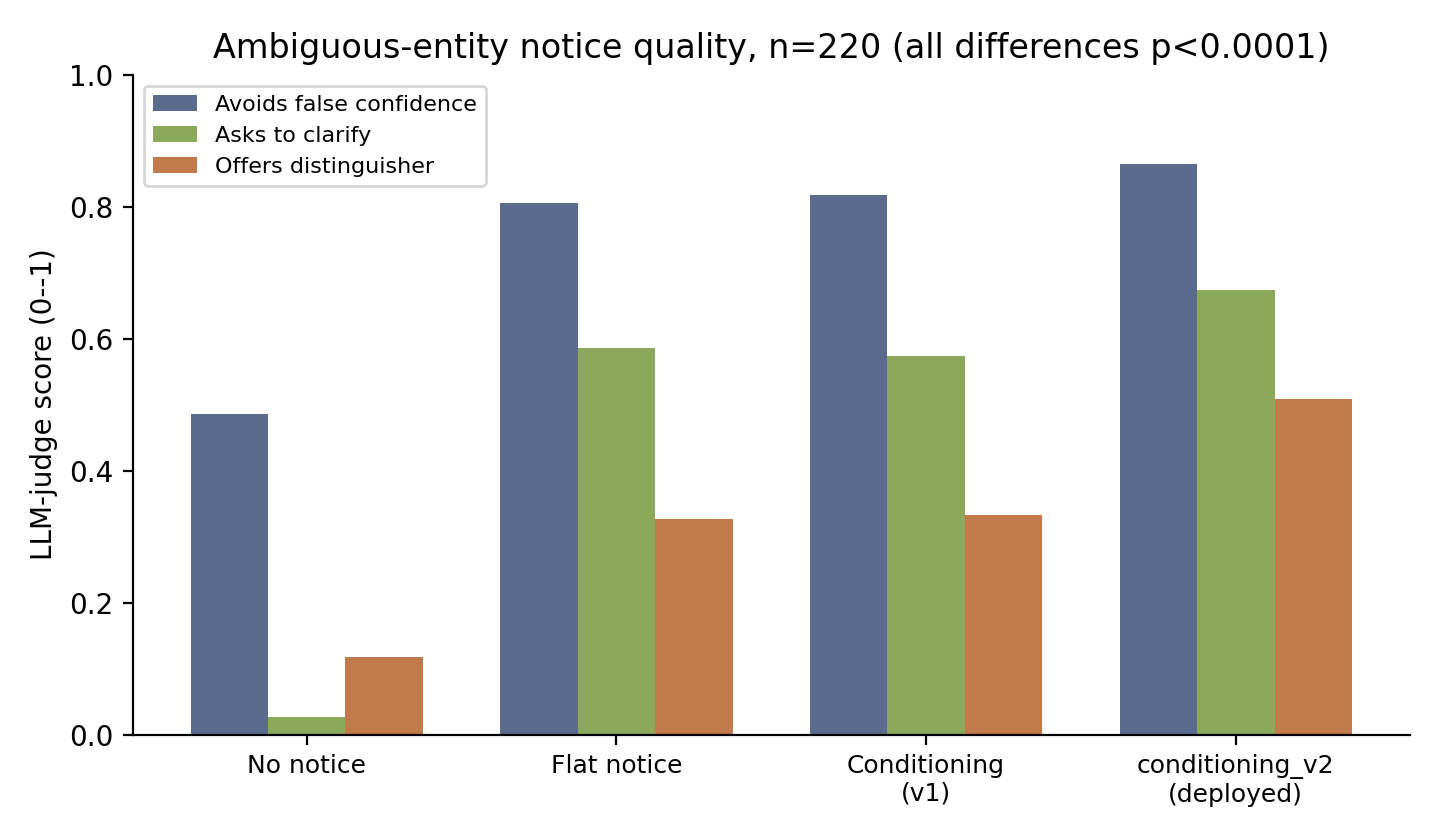
\includegraphics[width=8cm]{fig_conditioning_v2.png}}
\caption{Ambiguous-entity notice quality across all four tested conditions (same data as Table~\ref{tab:conditioning-v2-report}).}
\label{fig:conditioning-v2-report}
\end{figure}

A methodological note behind this result: an earlier significance pass using the original, holistic judge produced a striking but suspicious reversal (\texttt{conditioning\_v2} scoring worse on ``avoids false confidence''); manual inspection found textbook-correct clarifying questions being scored as failures, backwards relative to the criterion's own definition. Re-scoring with a validated, decomposed judge changed the verdict on 43.3\% of responses, reversing the apparent regression entirely -- reported here as a caution about automated LLM-judge reliability on nuanced criteria generally, not specific to this one result.

\textbf{Deconfounding-diagnostic methodology.} Adaptive routing's fusion-method choice for entity-heavy queries (Reciprocal Rank Fusion) tied a fixed linear-fusion baseline on the undisturbed test set -- an ambiguous result, since a separate exact-match ranking guarantee could have been masking a real deficit rather than confirming genuine parity. Temporarily removing that guarantee for one standalone diagnostic run resolved the ambiguity decisively (Table~\ref{tab:deconfound-report}): every single discordant query at Recall@1 and Recall@3 favored the fixed baseline, none favored the original RRF choice.

\begin{table}[h]
\caption{Deconfounding diagnostic: RRF vs.\ fixed linear-fusion baseline, ceiling removed.}\label{tab:deconfound-report}\centering
\begin{tabular}{|l|c|c|l|}
\hline
Metric & RRF & Fixed & Verdict \\
\hline
Recall@1 & 0.71 & 0.93 & 22/22 discordant, $p<0.0001$ \\
Recall@3 & 0.74 & 0.93 & 19/19 discordant, $p<0.0001$ \\
Recall@5 & 0.88 & 0.93 & 5/5 discordant, $p=0.063$ \\
\hline
\end{tabular}
\end{table}

\begin{figure}[h]
\centering
{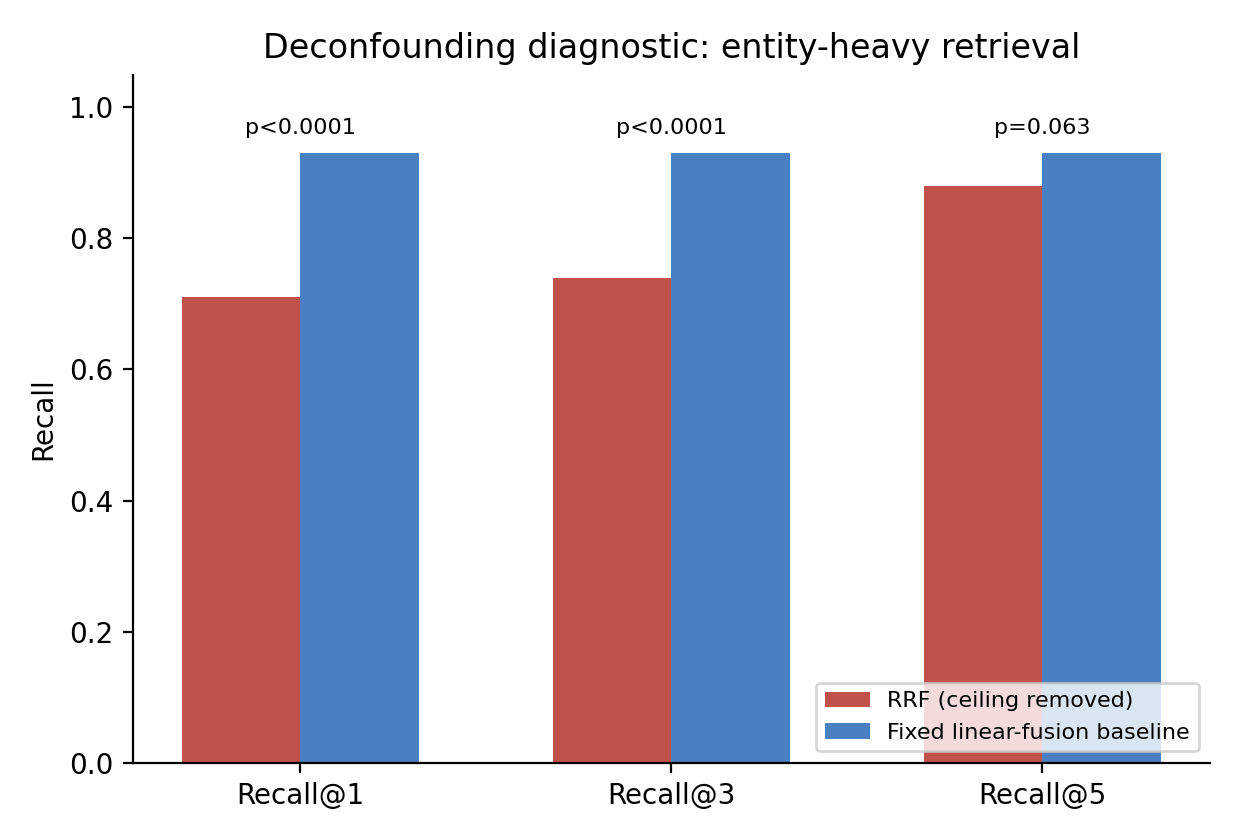
\includegraphics[width=7cm]{fig_deconfounding.png}}
\caption{Entity-heavy Recall@1/3/5 with the masking ranking guarantee removed (same data as Table~\ref{tab:deconfound-report}). Every discordant query at Recall@1 and Recall@3 favored the fixed baseline.}
\label{fig:deconfounding-report}
\end{figure}

The fix (replacing RRF with linear fusion at the same weighting) was then verified with the same diagnostic re-run: zero discordant pairs remained on Recall@1/3/5 against the fixed baseline -- not merely a restored tie, but genuine equivalence even without the masking guarantee's help.

\subsection{Confirmed Positive Component Results}
\label{subsec:results-positive-components}

Beyond the two novelty findings above, direct component ablation identifies exactly two components with a fully confirmed positive effect -- reported here with their real numbers rather than left as a qualitative claim, since a component-by-component ablation table does not make this pattern obvious on its own.

\textbf{Embedding fine-tuning.} Domain-adapting the retriever's sentence embeddings via contrastive training on this corpus's own (question, answer) pairs, evaluated on held-out validation data before deployment (never trained on): mining real hard negatives (actual retriever near-misses, not random text) beat in-batch-only contrastive training on both MRR ($0.536$ vs.\ $0.502$, paired bootstrap, $p=0.018$) and Top-1 accuracy ($0.290$ vs.\ $0.246$, $p=0.030$). A second retrain, following a data-ingestion pass that nearly tripled BanglishQA, was tested rather than assumed to help (more training data of a harder, noisier kind is not automatically an improvement): it produced a further significant MRR gain on the Banglish-only held-out set specifically ($+0.026$, $p=0.023$), with no significant regression on the pooled or structured-table held-out sets. Both gains were validated before, not after, full-pipeline deployment.

\textbf{Prerequisite-graph augmentation.} Multi-hop prerequisite-chain questions are answered by traversing a directed graph built from the \texttt{Prerequisites} table's own edge data, a query shape no single retrieved chunk can answer directly (Section~\ref{subsec:structured-tables}). Isolated ablation on an expanded $n=31$ sample of the corpus's own real, database-verified prerequisite chains (12 exercised by the main test set plus 19 additional real chains not previously tested) confirms a positive effect on all four generation-quality metrics, both paired tests agreeing throughout: BLEU ($+0.112$, $p=0.031$/$p=0.039$), ROUGE-L ($+0.094$, $p=0.026$/$p=0.042$), BERTScore ($+0.020$, $p=0.025$/$p=0.043$), and METEOR ($+0.071$, $p=0.034$/$p=0.039$). These figures were re-verified directly while preparing this report, prompted by a direct question about whether they were still current: an earlier measurement (predating a later Chroma-index rebuild that fixed a real bug elsewhere in the system) had reported a much larger effect ($p<0.0001$ on every metric); re-running the identical comparison found both conditions had improved since that fix, narrowing the gap substantially (graph-on now scores at or near ceiling, $1.000$/$1.000$/$1.000$/$0.999$) without eliminating the effect -- still significant on all four metrics, just more marginal than previously reported. This measurement has a further, older disclosed history: an earlier, smaller ($n=12$) test initially showed no effect, traced to a chunk-formatting bug (arrow vs.\ hyphen notation in stored chains) rather than genuine ineffectiveness; the bug, the fix, and this most recent re-verification are all reported, not only the most favorable number from any one round.

\textbf{Practical consequence: abstention rate.} The confidence-gated abstention mechanism (Section~\ref{subsec:results-abstention}), combined with the exact-match coverage fixes described in Section~\ref{subsec:process-arc}, reduces the system's rate of declining to answer to $0.5\%$ of English and $2.0\%$ of Banglish test queries, down from $10.5\%$ before the coverage fix -- a real, measured reduction in unnecessary refusals, not merely a design intention.

\subsection{Retrieval Quality}
\label{subsec:results-retrieval}

Reported separately for sparse (BM25-only), dense (vector-only), full hybrid, and adaptive routing, on the 200-query English test set. Recall@1/3/5, MRR, and nDCG@5/10 (paired bootstrap, adaptive vs.\ each baseline): adaptive ties full hybrid and BM25-only on all four metrics ($p\geq0.530$ both tests); against vector-only, three of four metrics tie and METEOR disagrees between tests ($p=0.128$ paired $t$, $p=0.018$ Wilcoxon) -- reported as inconclusive, not confirmed.

Precision@$k$ and MAP, computed with the identical relevance judgment used for Recall/MRR/nDCG (Table~\ref{tab:precision-map-report}), confirm the same parity ordering rather than surfacing a new finding.

\begin{table}[h]
\caption{Precision@$k$ and MAP, $n=200$.}\label{tab:precision-map-report}\centering
\begin{tabular}{|l|c|c|c|c|c|}
\hline
Config & P@1 & P@3 & P@5 & P@10 & MAP \\
\hline
Adaptive & 0.985 & 0.733 & 0.562 & 0.376 & 0.961 \\
Full hybrid & 0.985 & 0.730 & 0.564 & 0.376 & 0.960 \\
BM25-only & 0.975 & 0.715 & 0.551 & 0.371 & 0.952 \\
Vector-only & 0.965 & 0.660 & 0.501 & 0.315 & 0.897 \\
\hline
\end{tabular}
\end{table}

\subsection{Generation Faithfulness}
\label{subsec:results-faithfulness}

The RAGAS-style LLM-judge faithfulness score places the adaptive pipeline highest of four configurations (0.861); a matched-subset paired test finds this significant only against no-retrieval ($+0.236$, $p=0.007$), a non-significant tie against BM25-only/full-hybrid/vector-only.

An independent NLI-based faithfulness cross-check was tested across four models on the identical 169-row sample (Table~\ref{tab:nli-report}), each swap a genuine, separately-verified attempt rather than a single try.

\begin{table}[h]
\caption{NLI faithfulness cross-check, four models, identical sample.}\label{tab:nli-report}\centering
\begin{tabular}{|l|c|c|l|}
\hline
Model & Pearson $r$ & Agreement & Note \\
\hline
MiniLM (original) & $-0.300$ & 0.556 & chance-level \\
DeBERTa-base & $-0.076$ & 0.822 & improved, still negative \\
\textbf{DeBERTa-large-FEVER} & \textbf{$-0.018$} & \textbf{0.905} & best of four \\
MiniCheck & -- & -- & blocked, CVE-2025-32434 \\
\hline
\end{tabular}
\end{table}

Root cause of the remaining (near-zero, still negative) correlation was quantified rather than left unexplained: of 169 rows, 153 have both instruments agreeing the answer is faithful, and \emph{zero} have both agreeing it is unfaithful; 14 rows show the judge scoring high while NLI scores low (a structural blind spot on hedge/decline answers and on facts copied verbatim from structured multi-field records), and 2 show the reverse (at least one a confirmed LLM-judge scoring error, found by direct inspection). This asymmetry, not general disagreement, is what drives the negative sign. Two targeted fix attempts followed this diagnosis: excluding the single hedge-answer row moved $r$ from $-0.018$ to $-0.004$ (small, proportionate to the one affected row); re-splitting context by line as well as sentence (targeting the structured-record blind spot directly) made agreement \emph{worse} ($r=-0.245$), an honest negative result, not adopted.

\subsection{Abstention Gate}
\label{subsec:results-abstention}

The open-ended route's abstention gate progressed through three genuinely tested stages: a single-threshold gate (0.612 cross-validated accuracy) $\to$ a 4-signal logistic regression combining retrieval-score magnitudes with two structurally new signals, a lexical near-match check and a cross-stream (BM25/vector) agreement check (0.644, $+0.052$ over the threshold gate, $5/5$ independent fold seeds won) $\to$ a shallow gradient-boosted-tree ensemble over the same four signals (0.737). The final stage was deliberately scrutinized harder given how large the improvement looked: in-sample accuracy (0.873) shows a normal, moderate train/cross-validation gap rather than memorization, and the result is stable across five different classifier random seeds (0.7374--0.7390). The entity-heavy route's single-threshold gate was untouched throughout, already generalizing at 0.967 cross-validated accuracy.

This entire three-stage improvement was itself motivated by a methodological discovery, not attempted speculatively. The original threshold-selection procedure swept for the accuracy-maximizing threshold on the same set it then reported accuracy on, with no train/test split -- a reported 0.710 in-sample figure. A held-out re-validation (stratified 70/30 split, threshold selected on train only, evaluated on a test set never used for selection) found this gap was real and asymmetric: the entity-heavy route generalized well (0.944 held-out vs.\ in-sample), but the open-ended route did not (0.532 held-out, barely above chance on a class-balanced set). Because a single 70/30 split is itself sensitive to which points land in the test fold, the calibration was redone with full 5-fold cross-validation (0.612, Section~\ref{subsec:process-arc}), which is the actual baseline the subsequent two improvement stages were measured against. This same cross-validated re-calibration also surfaced a second, more subtle finding worth disclosing on its own terms: the entity-heavy route's own confidence signal is sharply bimodal on its calibration set (every value falls in $[0, 0.011]$ or $[99.98, 100.0]$, with no examples in between, a direct consequence of an unambiguous-match ranking ceiling), so a threshold anywhere in this wide empty gap scores identically on the available data -- cross-validation selected a threshold near the low end purely because of this degeneracy, not because it was a better choice, and the more conservative threshold near the ceiling was deployed instead. This is disclosed as a concrete illustration of why cross-validated threshold selection should not be trusted automatically without a sanity check against the mechanism being calibrated.

\subsection{Reranker Ablation}
\label{subsec:results-reranker}

Five configurations were tested, each a real, separately-measured attempt (Table~\ref{tab:reranker-report}); the deployed default remains reranker-off, since no configuration tested anywhere shows a measurable benefit.

\begin{table}[h]
\caption{Reranker configurations tested, in order.}\label{tab:reranker-report}\centering
\begin{tabular}{|l|l|}
\hline
Configuration & Result \\
\hline
Generic cross-encoder & Significant loss \\
Fine-tuned on hard negatives & Still a loss \\
Pool restricted (5 of 10) & Loss shrinks to noise \\
Route-conditional (open-ended only) & Clean tie vs.\ reranker-off \\
Route-conditional + pool-restricted & Null; adds nothing beyond route-conditional alone \\
\hline
\end{tabular}
\end{table}

Route-conditional reranking, additionally tested directly against the four external baselines (not only the reranker-off default): a clean tie against BM25-only and vector-only, and a borderline (test-disagreeing, hence inconclusive) result against full hybrid on two of four metrics -- a real nuance not previously documented, complementary to rather than contradicting the reranker-off tie.

\subsection{Efficiency}
\label{subsec:results-efficiency}

Latency was measured directly from per-query timing already logged on every evaluation run, isolating retrieval cost from generation cost (Table~\ref{tab:latency-report}). Retrieval is negligible in every configuration; generation dominates end-to-end cost, and the no-retrieval baseline shows a \emph{higher} median generation time, consistent with longer, less-grounded responses when no context is available to draw from.

\begin{table}[h]
\caption{Latency percentiles by stage (adaptive configuration).}\label{tab:latency-report}\centering
\begin{tabular}{|l|c|c|c|}
\hline
Stage & p50 & p95 & p99 \\
\hline
Retrieval & 20ms & 29ms & 35ms \\
Generation & 5.24s & 10.26s & 17.11s \\
\hline
\end{tabular}
\end{table}

\subsection{Robustness}
\label{subsec:results-robustness}

Consistency was measured directly: 20 real test queries (10 entity-heavy, 10 open-ended), each run three times independently through the full deployed pipeline. Retrieval was perfectly consistent (20/20 queries returned the identical top-1 document across all three repeats), confirming the cross-process determinism fix (Section~\ref{subsec:process-arc}) holds at a proper sample size, not only the single anecdotal query it was originally caught on. Generation, despite temperature $0.0$ and a fixed seed, was not perfectly deterministic: 17/20 queries (85\%) produced byte-identical answers across all three repeats, and the three that did not remained highly similar (mean minimum pairwise similarity $0.970$) rather than substantively different -- a direct, quantified measurement of a GPU floating-point non-determinism source previously noted only anecdotally.

\subsection{What Was Deliberately Not Attempted}
\label{subsec:not-attempted}

Three categories of measurement were considered and deliberately excluded, disclosed here rather than silently omitted. Standard external IR/QA benchmarks (BEIR, HotpotQA, MS MARCO) were not run: this system's claim is about a fixed, curated, single-institution bilingual corpus, and running a general-purpose web-scale benchmark would evaluate a different system's claims, not this one's. A scalability curve to corpus sizes far beyond this one's actual scale was likewise not attempted, for the same reason. Human evaluation was excluded per this report's own scope; machine-side preparation for a future annotation pass (a 50-item disagreement-prioritized sample between the LLM judge and the NLI cross-check) exists but the annotation itself requires a human rater. Finally, the main generation-quality metrics (BLEU/ROUGE-L/BERTScore/METEOR/faithfulness) are single-run rather than averaged over multiple generation seeds -- the calibration work in Section~\ref{subsec:results-abstention} does use 5 independent seeds, but re-running the full 300-query generation set multiple times was judged not to fit this report's scope; this is disclosed as a real limitation, not a silent gap.

\section{\uppercase{Limitations}}
\label{sec:limitations}

Honestly stated, in order of how directly each can be resolved by further engineering effort.

\textbf{No manual hallucination annotation.} The LLM-judge faithfulness score is a real, code-executed measurement, but it is a different instrument from human annotation against ground truth, uses a single automated judge with no second rater, and (Section~\ref{subsec:results-faithfulness}) does not fully agree with an independent NLI cross-check. This is the one limitation on this list that cannot be resolved by more engineering alone -- it requires an actual second human rater, outside this report's scope.

\textbf{The open-ended abstention gate, while substantially improved (0.612 $\to$ 0.737), is not the entity-heavy route's 0.967.} The remaining gap is real and disclosed, not hidden behind the headline improvement.

\textbf{Entity-heavy abstention calibration is capped at a genuine data ceiling.} Only 18 of 380 real out-of-scope/answerable rows in the database mention a course code or faculty name at all; the remainder of the 60-example calibration set is disclosed, database-verified synthetic augmentation, not additional organic data -- verified this project that no further real examples exist to add.

\textbf{The cross-lingual stress test is similarly capped}, at 13 real qualifying facts across both held-out splits combined, too small to significance-test with full confidence; its expanded (LLM-generated) 27-query version is not statistically significant on the current retriever.

\textbf{The reranker has never shown a measurable benefit}, in five separately-tested configurations (Section~\ref{subsec:results-reranker}); the best achievable state is a tie, not a win, and this is not expected to change without a fundamentally different reranker architecture.

\textbf{BM25-level Banglish spelling-variant normalization shows a null effect} on the main Banglish test set, a genuine tested-and-negative result, not an unexamined gap.

\textbf{The sufficient-context override is deliberately one-directional} -- it can only make the system less likely to abstain, never more, so it cannot itself compensate for a missed abstain-worthy query. This is a considered safety design, not a defect: forcing abstention on ambiguous evidence would risk declining to answer genuinely answerable questions.

\textbf{LLM-judge scoring is not safe to trust on nuanced, definition-sensitive criteria without a decomposed judge or cross-check} -- demonstrated directly in Section~\ref{subsec:results-novelty}'s judge-reliability correction (43.3\% of responses re-scored differently once a validated, decomposed judge replaced the original holistic one). This is a caution about the evaluation methodology generally, not specific to that one result.

\section{\uppercase{Conclusion}}
\label{sec:conclusion}

The dataset underlying this system is a real, provenance-labeled, bilingual corpus of 7{,}138 chunks with a naturally-occurring should-abstain label set, not a synthetic convenience sample. The process that produced the deployed system is a documented, chronological sequence of individually-verified fixes -- including a genuine methodological contribution (the deconfounding diagnostic) that turned an ambiguous tie into a diagnosed, fixed regression. The results reported here include two headline novelty findings, honest parity on standard automated metrics against single-method baselines, a three-stage abstention-gate improvement taken from 0.612 to 0.737 accuracy, and several honestly-reported negative results (a five-configuration reranker ablation and three of four faithfulness cross-check models) that did not improve on what came before them. Every number in this report traces to a script that produced it; nothing here is estimated.

\begin{thebibliography}{99}
\small

\bibitem[Dror et~al.(2018)]{dror2018hitchhiker} Dror, R., Baumer, G., Shlomov, S., and Reichart, R. (2018). The hitchhiker's guide to testing statistical significance in natural language processing. In \textit{Proceedings of the 56th Annual Meeting of the Association for Computational Linguistics}, pages 1383--1392.

\bibitem[Kruk et~al.(2025)]{kruk2025banglassist} Kruk, F., Herath, S., and Choudhury, P. (2025). BanglAssist: A Bengali-English generative AI chatbot for code-switching and dialect-handling in customer service. In \textit{Extended Abstracts of the CHI Conference on Human Factors in Computing Systems (CHI EA '25)}. arXiv:2503.22283.

\end{thebibliography}

\end{document}
